\documentclass{article}
\usepackage{tikz}
\usetikzlibrary{arrows.meta}

\begin{document}

\begin{center}
    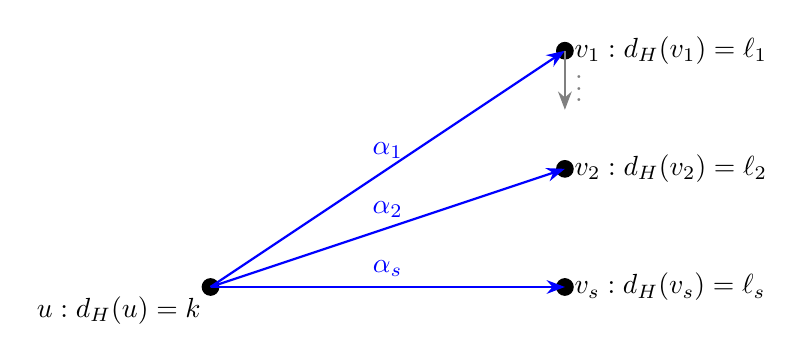
\begin{tikzpicture}[scale=1.5]
        % Define coordinates
        \coordinate (u) at (0,0);
        \coordinate (v1) at (3,2);
        \coordinate (v2) at (3,1);
        \coordinate (vs) at (3,0);

        % Draw nodes
        \filldraw[black] (u) circle (2pt) node[below left] {$u : d_H(u)=k$};
        \filldraw[black] (v1) circle (2pt) node[right] {$v_1 : d_H(v_1)=\ell_1$};
        \filldraw[black] (v2) circle (2pt) node[right] {$v_2 : d_H(v_2)=\ell_2$};
        \filldraw[black] (vs) circle (2pt) node[right] {$v_s : d_H(v_s)=\ell_s$};

        % Draw edges with labels
        \draw[blue, thick, -Stealth] (u) -- (v1) node[midway, above] {$\alpha_1$};
        \draw[blue, thick, -Stealth] (u) -- (v2) node[midway, above] {$\alpha_2$};
        \draw[blue, thick, -Stealth] (u) -- (vs) node[midway, above] {$\alpha_s$};

        % Draw vertical lines
        \draw[gray, thick, -Stealth] (v1) -- ++(0,-0.5) node[midway, right] {$\vdots$};
    \end{tikzpicture}
\end{center}

The multi-star \( S_{(k;\ell_1,\ldots,\ell_s;\alpha_1,\ldots,\alpha_s)}(H) \)

\end{document}